\documentclass[a4paper,oneside,DIV=12,12pt]{scrartcl}

\usepackage{graphicx}
\usepackage{float}

\usepackage{fontspec}
\setmainfont{STIX Two Text}
%\setsansfont{Roboto}
\newfontfamily{\cyrillicfontsf}{Roboto}
\setmonofont{PT Mono}

\usepackage{microtype}

\usepackage{polyglossia}
\setmainlanguage{ukrainian}

\usepackage{amsmath}
\usepackage{unicode-math}
\setmathfont{STIX Two Math}

% Load and set up dingbats font for X mark
\usepackage{pifont}
\newcommand{\xmark}{\ding{53}}
\newcommand{\xmarkbf}{\ding{54}}
%

\usepackage{IEEEtrantools}

\usepackage{karnaugh-map}

% Table typesetting
\usepackage{booktabs}

\usepackage{array}
\newcolumntype{v}[1]{>{\raggedright\arraybackslash\hspace{0pt}}p{#1}}
\newcolumntype{n}[1]{>{\raggedleft\arraybackslash\hspace{0pt}}p{#1}}

\usepackage{multirow}
%

\usepackage{tikz}
\usetikzlibrary{arrows,automata,positioning}

\usepackage{circuitikz}

\usepackage{siunitx}
\sisetup{output-decimal-marker = {,},
exponent-product = {\cdot}}

% Problem-solution typesetting
\usepackage{xsim}
\loadxsimstyle{runin}
\DeclareExerciseTranslations{exercise}{
	Ukrainian	=	завдання ,
}

\DeclareExerciseTranslations{solution}{
	Ukrainian	=	розв'язання ,
}

\xsimsetup{
	solution/print = true,
	exercise/template = runin,
	solution/template = runin,
}

% Count floats withing section
\usepackage{chngcntr}
\counterwithin{figure}{exercise}
\counterwithin{table}{exercise}
% End Count floats within section

\newcommand{\sheetno}[1]{{\centering\Large\bfseries Білет №#1\par}}

\renewcommand{\implies}{\rightarrow}

\newcommand\barneg[1]{\overline{#1}}
\newcommand{\logicequiv}{\leftrightarrow}
\newcommand{\lnor}{\mathbin{\downarrow}}

\newcommand{\langdef}[2]{#1~\textit{#2}}

\newcommand{\nbspthin}{\kern 1pt}

\begin{document}
	\begin{titlepage}
		\begin{center}
			Міністерство освіти і науки України\\
			Національний авіаційний університет\\
			Навчально-науковий інститут комп'ютерних інформаційних технологій\\
			Кафедра комп'ютеризованих систем управління
			
			\vspace{\fill}
				Академічна різниця\\
				з дисципліни:\\
				«Комп'ютерна логіка»\\
				I семестр
				
			\vspace{\fill}
			
			\begin{flushright}
				Виконав:\\
				студент ННІКІТ СП-225\\
				Клокун Владислав\\
			\end{flushright}
			Київ 2017
		\end{center}
	\end{titlepage}
	
	\sheetno{11}
	
	\begin{exercise}
		Опишіть логічні (булеві) функції від двох змінних.
	\end{exercise}
	
	\begin{solution}
		Булева функція від двох змінних --- це відображення $f\colon B^2 \mapsto B$, де $B = \{0, 1\}$. Для двох аргументів існує $2^{2^2} = 16$ можливих булевих функцій. Однак, найчастіше використовуються лише декілька. Розглянемо їх за допомогою таблиці істинності.
		
		\begin{table}[!htbp]
		\centering
			\begin{tabular}{ccccccc}
				\toprule
					    % &     & НЕ           & І & АБО \\
					$x$ & $y$ & $x \land y$ & $x \lor y$ & $x \implies y$ & $x \logicequiv y$ & $x \oplus y $\\
				\midrule
					0   & 0   & 0           & 0          & 1              & 1                 & 0\\
					0   & 1   & 0           & 1          & 1              & 0                 & 1\\
					1   & 0   & 0           & 1          & 0              & 0                 & 1\\
					1   & 1   & 1           & 1          & 1              & 1                 & 0\\
				\bottomrule
			\end{tabular}
		\caption{Таблиця істинності основних булевих функцій}
		\label{fig:bool-functioins-truth-table}
		\end{table}
	\end{solution}
	
	\begin{exercise}
		Побудувати таблицю істинності для функції $F$:
		\[
			F(x, y, z) = \left( \neg{(xy)} \implies z\right) \logicequiv \left( x \neg{z} \implies y \right).
		\]
	\end{exercise}
	
	\begin{solution}
		Таблиця істинності заданої функції наведена у табл.~\ref{tab:ex2-truth-table}.
		
		\begin{table}[!htbp]
		\centering
			\begin{tabular}{cccc}
				\toprule
					$x$ & $y$ & $z$ & $F(x, y, z)$\\
				\midrule
					0   & 0   & 0   & 0\\
					0   & 0   & 1   & 1\\
					0   & 1   & 0   & 1\\
					0   & 1   & 1   & 1\\
					1   & 0   & 0   & 0\\
					1   & 0   & 1   & 1\\
					1   & 1   & 0   & 1\\
					1   & 1   & 1   & 1\\
				\bottomrule
			\end{tabular}
		\caption{Таблиця істинності заданої функції}
		\label{tab:ex2-truth-table}
		\end{table}
	\end{solution}
	
	\begin{exercise}
		Виконайте спрощення логічного виразу~$L$ та мінімізацію логічного виразу~$F$, якщо:
		\[
			L = x_3x_2 \lor x_3 \barneg{x_2} \lor \barneg{\barneg{x_1} \lor \barneg{x_1 \lor x_2} },
		\]
		\[
			F = 0 \lor 4 \lor 7 \lor 8 \lor 11 \lor 12 \lor 13 \lor 15.
		\]
	\end{exercise}
	
	\begin{solution}
		Спростимо логічний вираз $L$, використовуючи закони Де~Моргана, подвійного заперечення, ідемпотенції та дистрибутивності.
		\begin{IEEEeqnarray*}{rCl}
			%L &=& x_3x_2 \lor x_3 \barneg{x_2} \lor \barneg{\barneg{x_1} \lor \barneg{x_1 \lor x_2} }\\
			%  &=& x_3 x_2 \lor x_3 \barneg{x_2} \lor \barneg{\barneg{x_1}} \barneg{\barneg{(x_1 \lor x_2)}}\\
			%  &=& x_3 x_2 \lor x_3 \barneg{x_2} \lor x_1 x_1 \lor x_2\\
			%  &=& x_3 x_2 \lor x_3 \barneg{x_2} \lor x_1 x_1 \lor x_1 x_2\\
			%  &=& x_3 (x_2 \lor \barneg{x_2}) \lor x_1 \lor x_1 x_2\\
			%  &=& x_3 \lor x_2 \lor x_1(1 + x_2)\\
			%  &=& x_3 \lor x_1.
			%  
			L &=& x_3 \land x_2 \lor x_3 \land \neg x_2 \lor \neg (\neg x_1 \lor \neg(x_1 \lor x_2)\\
			  &=& x_3 \land x_2 \lor x_3 \land \neg x_2 \lor \neg (\neg x_1) \land \neg(\neg (x_1 \lor x_2))\\
			  &=& x_3 \land x_2 \lor x_3 \land \neg x_2 \lor x_1 \land (x_1 \lor x_2)\\
			  &=& x_3 \land x_2 \lor x_3 \land \neg x_2 \lor x_1 \land x_1 \lor x_1 \land x_2\\
			  &=& x_3 \land (x_2 \lor \neg x_2) \lor x_1 \lor x_1 \land x_2\\
			  &=& x_3 \lor x_1 \lor x_1 \land x_2\\
			  &=& x_3 \lor x_1 \land (1 \lor x_2)\\
			  &=& x_3 \lor x_1.
		\end{IEEEeqnarray*}
		
		Мінімізуємо логічний вираз $F$. Для цього представимо його у двійковому вигляді:
		\begin{IEEEeqnarray*}{rCl}
			F &=& 0 \lor 4 \lor 7 \lor 8 \lor 11 \lor 12 \lor 13 \lor 15\\
			  &=& 0000 \lor 0100 \lor 0111 \lor 1000 \lor 1011 \lor 1100 \lor 1101 \lor 1111\\
			  &=& \neg{A} \neg{B} \neg{C} \neg{D}
			      \lor \neg{A}      B \neg{C} \neg{D}
			      \lor \neg{A}      B  \neg{C} \neg{D}
			      \lor \neg{A}      B       C       D \\
			  &&  \lor      A  \neg{B} \neg{C} \neg{D}
			      \lor      A  \neg{B}      C       D
			      \lor      A       B  \neg{C}      D
			      \lor      A       B       C       D.
		\end{IEEEeqnarray*}
		
		Побудуємо карту Карно (рис.~\ref{fig:task3-karnaugh-map}).
		\begin{figure}
		\centering
			\begin{karnaugh-map}*[4][4][1][$CD$][$AB$]
				\minterms{0,4,7,8,11,12,13,15}
				\implicant{0}{8}
				\implicant{13}{15}
				\implicant{ 7}{15}
				\implicant{15}{11}
			\end{karnaugh-map}
		\caption{Карта Карно логічного виразу $F$}
		\label{fig:task3-karnaugh-map}
		\end{figure}
		Звідси маємо:
		\[
			F = \neg{C} \neg{D} \lor ABD \lor BCD \lor ACD.
		\]
	\end{solution}
	
	\begin{exercise}
		Отримати МДНФ перемикальної функції, що задана діаграмою Вейча (рис.~\ref{fig:task4-veitch-diagram}). Для мінімізації застосувати метод Квайна\nbspthin —\nbspthin МакКласкі. Перемикальну функцію реалізувати в елементному базисі АБО---НЕ.
		
		\begin{figure}[!htbp]
		\centering
			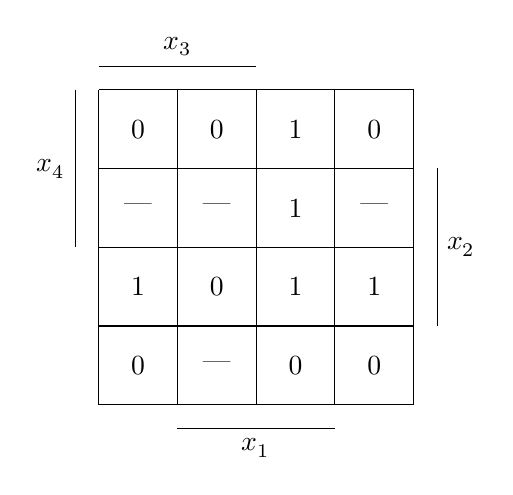
\begin{tikzpicture}
				\draw (0,0) grid (4,4);
				\node at (0.5,0.5){0};
				\node at (1.5,0.5){—};
				\node at (2.5,0.5){0};
				\node at (3.5,0.5){0};

				\node at (0.5,1.5){1};
				\node at (1.5,1.5){0};
				\node at (2.5,1.5){1};
				\node at (3.5,1.5){1};
				
				\node at (0.5,2.5){—};
				\node at (1.5,2.5){—};
				\node at (2.5,2.5){1};
				\node at (3.5,2.5){—};
				
				\node at (0.5,3.5){0};
				\node at (1.5,3.5){0};
				\node at (2.5,3.5){1};
				\node at (3.5,3.5){0};
				
				\draw (0,4.3) --node[midway, above]{$x_3$} (2,4.3);
				\draw (-0.3,4) --node[midway, left]{$x_4$} (-0.3,2);
				\draw (1,-0.3) --node[midway, below]{$x_1$} (3,-0.3);
				\draw (4.3,1) --node[midway, right]{$x_2$} (4.3,3);
			\end{tikzpicture}
		\caption{Діаграма Вейча заданої перемикальної функції}
		\label{fig:task4-veitch-diagram}
		\end{figure}
		
	\end{exercise}
	
	\begin{solution}
		Нехай задана перемикальна функція $f(x_1, x_2, x_3, x_4)$, тоді побудуємо таблицю істинності~(табл.~\ref{tab:task4-function-truth-table}) за діаграмою Вейча заданої функції~(рис.~\ref{fig:task4-veitch-diagram}).
		
		\begin{table}[!htbp]
		\centering
			\begin{tabular}{ccccc}
				\toprule
					$x_1$ & $x_2$ & $x_3$ & $x_4$ & $f(x_1, x_2, x_3, x_4)$ \\
				\midrule
					0     & 0     & 0     & 0     & 0 \\
					0     & 0     & 0     & 1     & 0 \\
					0     & 0     & 1     & 0     & 0 \\
					0     & 0     & 1     & 1     & 0 \\
					0     & 1     & 0     & 0     & 1 \\
					0     & 1     & 0     & 1     & — \\
					0     & 1     & 1     & 0     & 1 \\
					0     & 1     & 1     & 1     & — \\
					1     & 0     & 0     & 0     & 0 \\
					1     & 0     & 0     & 1     & 1 \\
					1     & 0     & 1     & 0     & — \\
					1     & 0     & 1     & 1     & 0 \\
					1     & 1     & 0     & 0     & 1 \\
					1     & 1     & 0     & 1     & 1 \\
					1     & 1     & 1     & 0     & 0 \\
					1     & 1     & 1     & 1     & — \\
				\bottomrule
			\end{tabular}
		\caption{Таблиця істинності заданої функції $f(x_1, x_2, x_3, x_4)$}
		\label{tab:task4-function-truth-table}
		\end{table}
		
		Запишемо функцію у вигляді досконалої диз'\-юн\-ктив\-ної нормальної форми (ДДНФ) двійкових представлень.
		\[
			f(x_1, x_2, x_3, x_4) = 0100 \lor 0110 \lor 1001 \lor 1100 \lor 1101.
		\]
		
		Складемо таблицю мінтермів~(табл.~\ref{tab:task4-minterm-table}). Для виконання мінімізації внесемо до неї не тільки мінтерми, а й терми, значення яких нас не цікавить (\langdef{англ.}{don't-care terms}).
		
		\begin{table}[!htbp]
		\centering
			\begin{tabular}{v{5em}ln{7em}}
				\toprule
					Кількість одиниць & Мінтерм & Двійкове представлення\\
				\midrule
					1           & \texttt{m04}      & \texttt{0100}\\
					\cmidrule(lr){1-3}
					\multirow{5}{*}{2}
					            & \texttt{m06}      & \texttt{0110}\\
					            & \texttt{m09}      & \texttt{1001}\\
					            & \texttt{m12}      & \texttt{1100}\\
					            & \texttt{d05}      & \texttt{0101}\\
					            & \texttt{d10}      & \texttt{1010}\\
					\cmidrule(lr){1-3}
					\multirow{2}{*}{3}
					            & \texttt{m13}      & \texttt{1101}\\
					            & \texttt{d07}      & \texttt{0111}\\
					\cmidrule(lr){1-3}
					4           & \texttt{d15}      & \texttt{1111}\\
				\bottomrule
			\end{tabular}
		\caption{Таблиця мінтермів}
		\label{tab:task4-minterm-table}
		\end{table}
		
		Побудуємо таблицю для пошуку простих імплікант~(табл.~\ref{tab:task4-finding-prime-implicants}). Прості імпліканти виділені жирним шрифтом.
		
		\begin{table}[!htbp]
		\centering
			\begin{tabular}{v{5em}cccccc}
				\toprule
					Кількість одиниць & Мінтерм & & \multicolumn{2}{c}{2-імпліканти} & \multicolumn{2}{c}{4-імпліканти}\\
				\midrule
					\multirow{3}{*}{1}
						& \texttt{m04}          & \texttt{0100}          & \texttt{(m04,m06)}          & \texttt{01—0}          & \strong{\texttt{(m04,m06,d05,d07)}} & \strong{\texttt{01——}}\\
						&                       &                        & \texttt{(m04,m12)}          & \texttt{—100}          & \strong{\texttt{(m04,m12,m13,d05)}} & \strong{\texttt{—10—}}\\
						&                       &                        & \texttt{(m04,d05)}          & \texttt{010—}          &                                     &  \\
					\cmidrule(lr){1-7}
					\multirow{6}{*}{2}
						& \texttt{m06}          & \texttt{0110}          & \texttt{(m06,d07)}          & \texttt{011—}          & \strong{\texttt{(m13,d05,d07,d15)}} & \strong{\texttt{—1—1}}\\
						& \texttt{m09}          & \texttt{1001}          & \strong{\texttt{(m09,m13)}} & \strong{\texttt{1—01}} &                                     & \\
						& \texttt{m12}          & \texttt{1100}          & \texttt{(m12,m13)}          & \texttt{110—}          &                                     & \\
						& \texttt{d05}          & \texttt{0101}          & \texttt{(d05,m13)}          & \texttt{—101}          &                                     & \\
						&                       &                        & \texttt{(d05,d07)}          & \texttt{01—1}          &                                     & \\
						& \strong{\texttt{d10}} & \strong{\texttt{1010}} &                             &                        &                                     & \\
					\cmidrule(lr){1-7}
					\multirow{2}{*}{3}
						& \texttt{m13}          & \texttt{1101}          & \texttt{(m13,d15)}          & \texttt{11—1}          &                                     & \\
						& \texttt{d07}          & \texttt{0111}          & \texttt{(d07,d15)}          & \texttt{—111}          &                                     & \\
					\cmidrule(lr){1-7}
					\multirow{1}{*}{4}
						& \texttt{d15}          & \texttt{1111}          &                             &                        &                                     & \\
				\bottomrule
			\end{tabular}
		\caption{Таблиця пошуку простих імплікант}
		\label{tab:task4-finding-prime-implicants}
		\end{table}
		
		Складаємо таблицю простих імплікант (табл.~\ref{tab:task4-coverage-table}). До неї заносимо лише ті виходи функції, які мають значення. Ядрами будуть ті значення, у рядках яких існує лише одне перекриття.
		
		\begin{table}[!htbp]
		\centering
			\begin{tabular}{lcccc}
				\toprule
					& \texttt{01——} & \texttt{—10—} & \texttt{—1—1} & \texttt{1—01} \\
				\midrule
				\texttt{m04}  &  \xmark       & \xmark        &               &               \\
				\texttt{m06}  &  \xmarkbf     &               &               &               \\
				\texttt{m09}  &               &               &               & \xmarkbf      \\
				\texttt{m12}  &               & \xmarkbf      &               &               \\
				\texttt{m13}  &               & \xmark        & \xmark        & \xmark        \\
				\bottomrule
			\end{tabular}
		\caption{Таблиця покриття}
		\label{tab:task4-coverage-table}
		\end{table}
		
		Таким чином за методом Квайна\nbspthin —\nbspthin МакКласкі отримали МДНФ такого вигляду:
		\[
			f (x_1, x_2, x_3, x_4) = x_1 \land \neg{x_3} \land x_4 \lor x_2 \land \neg{x_3} \lor \neg{x_1} \land x_2.
		\]
		
		Переходимо у базис АБО—НЕ:
		\begin{IEEEeqnarray*}{rCl}
			f (x_1, x_2, x_3, x_4) &=& x_1 \land \neg{x_3} \land x_4 \lor x_2 \land \neg{x_3} \lor \neg{x_1} \land x_2\\
			                       &=& (\neg{x_1} \lnor \neg{x_3}) \lnor (x_1 \lnor x_2) \lnor (x_2 \lnor x_4).
		\end{IEEEeqnarray*}
		
		Реалізуємо отриману перемикальну функцію~(рис.~\ref{fig:task4-schematic}).
		
		\begin{figure}[!htbp]
		\centering
			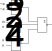
\includegraphics[]{task4-schematic.pdf}
		\caption{Схема отриманої перемикальної функції}
		\label{fig:task4-schematic}
		\end{figure}
		
	\end{solution}
	
	\begin{exercise}
		За даним графом автомата~(рис.~\ref{fig:task5-automata-graph}) виконати синтез керуючого автомата. Для побудови функціональної схеми використати T-тригери. Елементний базис: І, АБО, НЕ.
		
		\begin{figure}[!htbp]
		\centering
			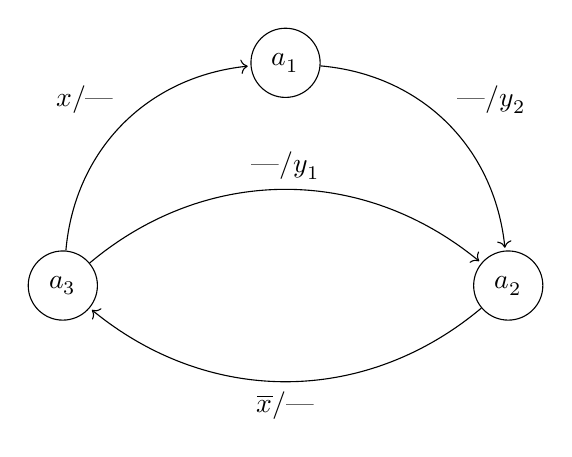
\begin{tikzpicture}[shorten >=1pt,node distance=4cm,on grid,auto]
				
				\node[state]	(a_1)		{$a_1$};
				\node[state]	(a_2) [below right=of a_1]	{$a_2$};
				\node[state]	(a_3) [below left=of a_1]	{$a_3$};
				
				\path[->]	(a_1)	edge [bend left=40]	node {$— / y_2$}	(a_2)
							(a_2)	edge [bend left=40]	node {$\barneg{x} / —$}				(a_3)
							(a_3)	edge [bend left=40]	node {$x / —$}		(a_1)
									edge [bend left=40]	node {$— / y_1$}	(a_2);
				
			\end{tikzpicture}
		\caption{Граф даного автомата Мілі}
		\label{fig:task5-automata-graph}
		\end{figure}
		
	\end{exercise}
\end{document}